\documentclass[a4paper,11pt]{article}
\usepackage[latin1]{inputenc}
\usepackage[T1]{fontenc}
\usepackage{amsmath}
\usepackage{amsfonts}
\usepackage{a4wide}
\usepackage{booktabs}
\usepackage{graphicx}
\usepackage{url}
\RequirePackage{color}

\newcommand{\red}{\color[rgb]{.9,0.1,0.1}}
\renewcommand{\epsilon}{\varepsilon}

\title{Genomics and Bioinformatics}
\date{December 17, 2013}
\author{Exam correction}
\begin{document}
\maketitle

\section*{Question 1 - Phylogenetic trees}

\begin{figure}[h!]
\centering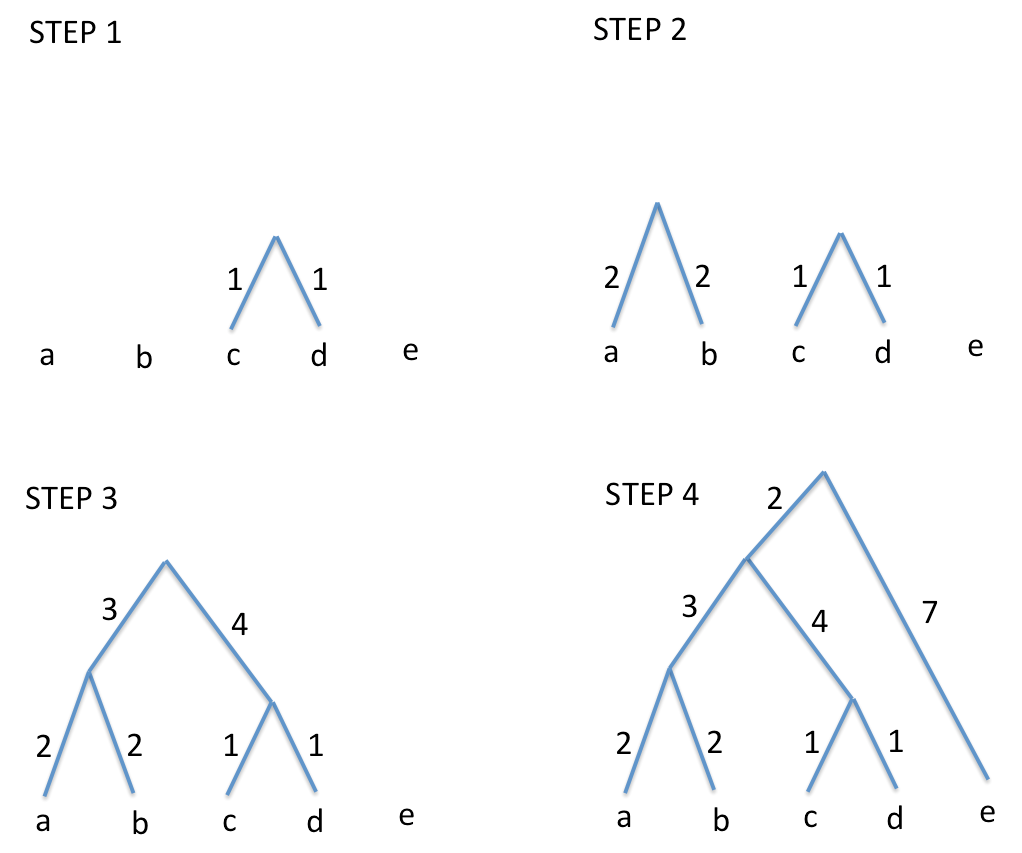
\includegraphics[width=14cm]{UPGMA.png}
\end{figure}

\section*{Question 2 - Linear models}


\begin{enumerate}
\item Assign value $0$ to ``untreated'' and $1$ to ``treated''.
The model can be written $Y = \text{a} + bT + \epsilon$, where
$Y \in \mathbb{R}^{12}$ are the probe intensities, 
$\text{a} = (a,...,a)' \in \mathbb{R}^{12}$ is the intercept, 
$b \in \mathbb{R}$ is the coefficient measuring the effect on $Y$ of varying $T$, 
$T \in \mathbb{R}^{12}$ is the binary vector ``treated/untreated'', 
$\epsilon \in \mathbb{R}^{12}$ is the measurement error.

\noindent
In matrix form:
$$
\left(
\begin{array}{c}
166\\121\\166\\270\\39\\121\\10\\14\\24\\14\\10\\3
\end{array}
\right)
=
\left(
\begin{array}{cc}
1 & 1 \\ 1 & 1 \\ 1 & 1 \\ 1 & 1 \\ 1& 1 \\ 1 & 1 \\ 1 & 0 \\ 1 & 0 \\ 1 & 0 \\ 1 & 0 \\ 1 & 0 \\ 1 & 0
\end{array}
\right)
\left(
\begin{array}{c}
a \\ b
\end{array}
\right)
+
\left(
\begin{array}{c}
\epsilon_1 \\ \epsilon_2 \\ \epsilon_3 \\ \epsilon_4 \\ \epsilon_5 \\ \epsilon_6 \\ \epsilon_7 \\ \epsilon_8 \\ \epsilon_9 \\ 
\epsilon_{10} \\ \epsilon_{11} \\ \epsilon_{12} 
\end{array}
\right) ,
$$
or $Y = X \beta + \epsilon$.

\item \begin{itemize}
	\item The p-value 0.00488 from the table is by definition the probability to observe an even bigger effect in the future, 
	given our data, under the null hypothesis. That is, it will happen randomly 5 times out of 1000 under the null, 
	which can -arguably- be considered as a rare event.
	So we can consider significant the effect of B.
	\item The expected increase in intensity is the estimate of $b$, 57.83.
	\end{itemize}
\item The normalized table:

\begin{table}[h!]
\centering
\begin{tabular}{l | cccccc}
   & P1 & P2 & P3 & P4 & P5 & P6\\
\hline
A & 90   & 60   & 90  & 140 & 20 & 60 \\
B & 60   & 60   & 90  & 140 & 20 & 90 \\
C & 60   & 90   & 140 & 90  & 60 & 20 \\  
\end{tabular}
\end{table}

\end{enumerate}

\section*{Question 3 - Transcription}

\begin{enumerate}
\item RNA-seq detects fragments of mature RNA, which do not contain
  introns due to splicing. On the other hand, NET-seq is able to
  detect nascent trancripts before being spliced and modified. This is
  why we can see peaks in introns in the NET-seq data, but not the
  RNA-seq data. 
\item We can deduce from figure 2d that there is a positive
  correlation between histone H4 hyperacetylation and antisense
  transcription. 
\item
	\begin{itemize}
	\item Loss of RCO1 should lead to more acetylation, and
          therefore more antisense transcription. 
	\item Figure 3b shows this effect on a genome-wide level. We
          can see that loss of RCO1 leads to a generally higher
          antisense/sense ratio. 
	\end{itemize}
%\item There is no effect of alpha-aminitin on the RNAPII density. The
%  authors use this assay to see if any transcription is proceeding
%  after the cells have been lysed in preparation for nascent RNA
%  extraction. 
\end{enumerate}

\section*{Question 4 - DNA Binding}


\begin{enumerate}
\item Consensus: \texttt{CATG} (score=$4$)
\item The next best sequences are \texttt{CCTG}, \texttt{CAGG} (score=$3.5$)
\item The scores are, with the best score and motif in red:
$$
\begin{matrix}
\bf A&\bf T&\bf A&\bf G&\red{\bf C}&\red{\bf C}&\red{\bf T}&\red{\bf A}&\bf G\cr
-6.28&0.5&-7.28&-3.64&\red{1.5}&-4.28&\phantom{0.00}&\phantom{0.00}&\phantom{0.00}
\end{matrix}
$$
%\item Using the background nucleotide frequencies:
%$$
%\begin{matrix}
%\bf A&\bf T&\bf A&\bf G&{\bf C}&{\bf C}&{\bf T}&{\bf A}&\bf G\cr
%-7.47&-1.96&-11.01&-7.37&-0.96&-6.74&\phantom{0.00}&\phantom{0.00}&\phantom{0.00}
%\end{matrix}
%$$
\item The scores of the motifs are $W(\texttt{CATG})=4$ and
  $W(\texttt{CTGG})=-0.64$ therefore the ratio of the number of proteins binding to
  each motif is:
$$
\frac{n(\texttt{CTGG})}{n(\texttt{CATG})}\,=\,\frac{1000\cdot e^{-0.64}}{e^4}
\,=\,1000\cdot e^{-4.64}~.
$$
This leads to the following proportion
$$
\frac{n(\texttt{CATG})}{n(\texttt{CATG})+n(\texttt{CTGG})}\,=\,\frac
1{1+1000\cdot e^{-4.64}}\,=\,\frac 1{11}.~
$$
\end{enumerate}

\end{document}
